 \chapter{Introduction}
\label{chap:introduction}

The optical frequency comb is a versatile tool for science and technology. Its invention two decades ago initiated a revolution in precision measurement by dramatically improving the resolution with which we can conveniently measure time and frequency \cite{Diddams2000,Jones2000,Diddams2001,Udem2002,Hall2006,Hansch2006}. This revolution was brought about by a combination of high performing femtosecond laser technology such as the modelocked Ti:sapphire laser \cite{Stingl1995} and new methods for tailoring the fundamental nonlinear interaction between light and matter \cite{Ranka2000,Dudley2006}. This powerful combination enabled the generation of laser pulse trains with coherent, octave-spanning spectra, which allowed implementation of a simple scheme by which the hundreds-of-terahertz-scale optical frequencies making up the laser could be measured electronically, as described below in Sec. \ref{sec:f2f}. Since their introduction, optical frequency combs have found important roles in many contexts. These range from investigation of basic scientific questions such as the time-variation of fundamental constants \cite{Lea2007,Blatt2008} and the size of the proton \cite{Beyer2017} to applications such as systems for ultra-low-noise microwave synthesis \cite{McFerran2005,Fortier2011}, broadband spectroscopy \cite{Diddams2007,Coddington2016}, optical arbitrary waveform generation \cite{Cundiff2010}, and stable long-term calibration of astronomical spectrographs for exoplanet detection \cite{Steinmetz2008}. Further development of the technology beyond the first stabilization of the Ti:sapphire laser that heralded the frequency comb's arrival has enabled combs to reach applications across many wavelength bands \cite{Washburn2004a,Gohle2005b,Diddams2010,Faist2016}, and in particular modelocked fiber-laser frequency combs have proven to be versatile, compact systems that are useful for many applications \cite{Newbury2007,Fermann2013,Sinclair2015}. The technology is reaching maturity: frequency combs have been deployed outside the laboratory for spectroscopy applications \cite{Sinclair2014,Coburn2018}, and space-borne comb operation has been demonstrated in microgravity conditions during the flight of a sounding rocket \cite{Lezius2016}. Packaged frequency combs have been commercially available as laboratory tools for some time.

In the last decade, methods for generating optical frequency combs without a modelocked laser have emerged. These new frequency combs come with higher repetition rates and lower fundamental size, weight, and power (SWAP) requirements. Higher repetition rates make them particularly attractive for applications where high power per comb mode, individual accessibility of comb modes, and fast acquisition times are desired; these applications include arbitrary microwave and optical waveform generation, telecommunications, and broadband, temporally-resolved spectroscopy. With their low SWAP requirements these combs present a promising route towards planar integration of frequency combs, which could enable their seamless inclusion in compact devices for applications outside the laboratory and will continue to drive forward the revolution that was initiated some twenty years ago. There remains much work to be done, however, to develop these combs that are based on continuous-wave lasers to the level of technological maturity that has been reached by modelocked-laser-based combs.

%begun to suggest new ways to bring their capabilities to applications outside the controlled environment of the research laboratory.

%These combs are beginning, enabling e.g. direct optical frequency synthesis on a chip \cite{Spencer2018}.

%which could well lead to a second revolutionMoreover, these combs come with lower fundamental size, weight, and power (SWAP) requirements, which will enable them to provide the features that make modelocked-laser-based combs attractive in a more portable package. 

This thesis focuses on these new frequency combs, with several related, discrete areas of focus. The bulk of the thesis covers microresonator-based frequency combs (microcombs), and especially the nonlinear dynamics involved in the generation of these frequency combs via the Kerr nonlinearity. An introduction to this field is provided in Chapter \ref{chap:microresonators}. Chapters \ref{chap:PMPumping}-\ref{chap:FPLLE} describe advancements in the field, and Chapter \ref{chap:conclusion} provides a brief summary and a discussion of avenues for further research on this topic. Then, Chapter \ref{chap:EOMCombs} presents a second method for generating a high-repetition-rate frequency comb without modelocking that is based on active modulation of a CW seed laser and subsequent nonlinear spectral broadening. The first self-referencing of a comb of this type is described, and a proof-of-principle application to the generation of low-noise microwaves is discussed. An outlook for further development of this type of comb is presented. Finally, in Chapter \ref{chap:PulsePicking}, I present experimental and theoretical investigations of repetition-rate reduction of frequency combs via pulse gating, which may prove useful for adapting low-SWAP combs and their intrinsically high repetition rates to some applications as the technology continues to develop. 

In the remainder of this chapter, I discuss the basic properties of frequency combs and explain how the optical frequencies making up a comb can be fully determined by electronics operating with gigahertz-scale bandwidths.

\section{Optical frequency combs}

An optical frequency comb is obtained by fully stabilizing the spectrum of an optical pulse train. The first frequency combs came about through full frequency-stabilization of modelocked lasers, which are multi-mode lasers in which the co-lasing modes are made to synchronize and generate a train of pulses. This is achieved through the introduction of a modelocking mechanism that lowers loss for pulsed operation; such mechanisms include spatial Kerr self-focusing \cite{Spence1991,Brabec1992}, nonlinear polarization rotation \cite{Hofer1992,Fermann1993}, and saturable absorption \cite{Stankov1988}. This thesis focuses on frequency comb pulse trains that are generated through other means. In particular, these combs are derived from a continuous-wave laser that functions as the central mode of the comb without the use of a cavity with broadband active gain. 

\subsection{Optical pulse trains and their spectra}

In the time domain, a frequency comb consists of a train of uniformly spaced optical pulses arriving at the pulse train's repetition rate $f_{rep}$, which within the growing space of frequency comb technology is between $\sim$10 MHz and $\sim$1 THz; the combs discussed in this thesis have repetition rates between 10 GHz and 30 GHz. In most implementations the pulses are very short compared to the repetition period $T=1/f_{rep}$, with durations on the order of 100 fs. In the frequency domain, the comb consists of a set of modes that are spaced by $f_{rep}$ in frequency and that have amplitudes determined by an overall spectral envelope centered at the optical carrier frequency $\nu_c$ ($\sim$193 THz in this thesis), with bandwidth inversely related to the temporal duration of the pulses. The usual description of a frequency comb, which is natural for modelocked-laser-based combs that are not derived from a CW laser, gives the frequencies of the comb modes as 
\begin{equation}
\nu_n=nf_{rep}+f_0, \label{eq:combfreqsold}
\end{equation} 
where $n\sim \nu_c/f_{rep}$ for the optical modes that make up the comb and $f_0$ is the carrier-envelope offset frequency, which may be defined to be between $0$ and $f_{rep}$. The offset frequency results from the pulse-to-pulse evolution of the carrier wave underneath the temporal intensity envelope of the pulses due to a difference in group and phase velocities. An equivalent representation of the frequencies of the comb that is more natural for frequency combs directly derived from a CW laser, as described in this thesis, is
\begin{equation}
\nu_\mu=\nu_c+\mu f_{rep}, \label{eq:combfreqsnew}
\end{equation} 
where $\nu_c$ is the frequency of the CW laser, the `pump' or `seed' laser, from which the frequency comb is derived and $\mu$ is a pump-referenced mode number, in contrast with the zero-referenced mode number $n$ of Eq. \ref{eq:combfreqsold}. Now the carrier-envelope offset frequency $f_0$ is found in the difference between $\nu_c$ and the closest harmonic of $f_{rep}$: $f_0=\nu_c-N f_{rep}$, where $N$ is the largest integer such that $f_0>0$. Fig. \ref{fig:CombBasics} depicts the properties of a frequency comb in the time domain and the frequency domain.

\begin{figure}[htpb]
	\begin{center}
		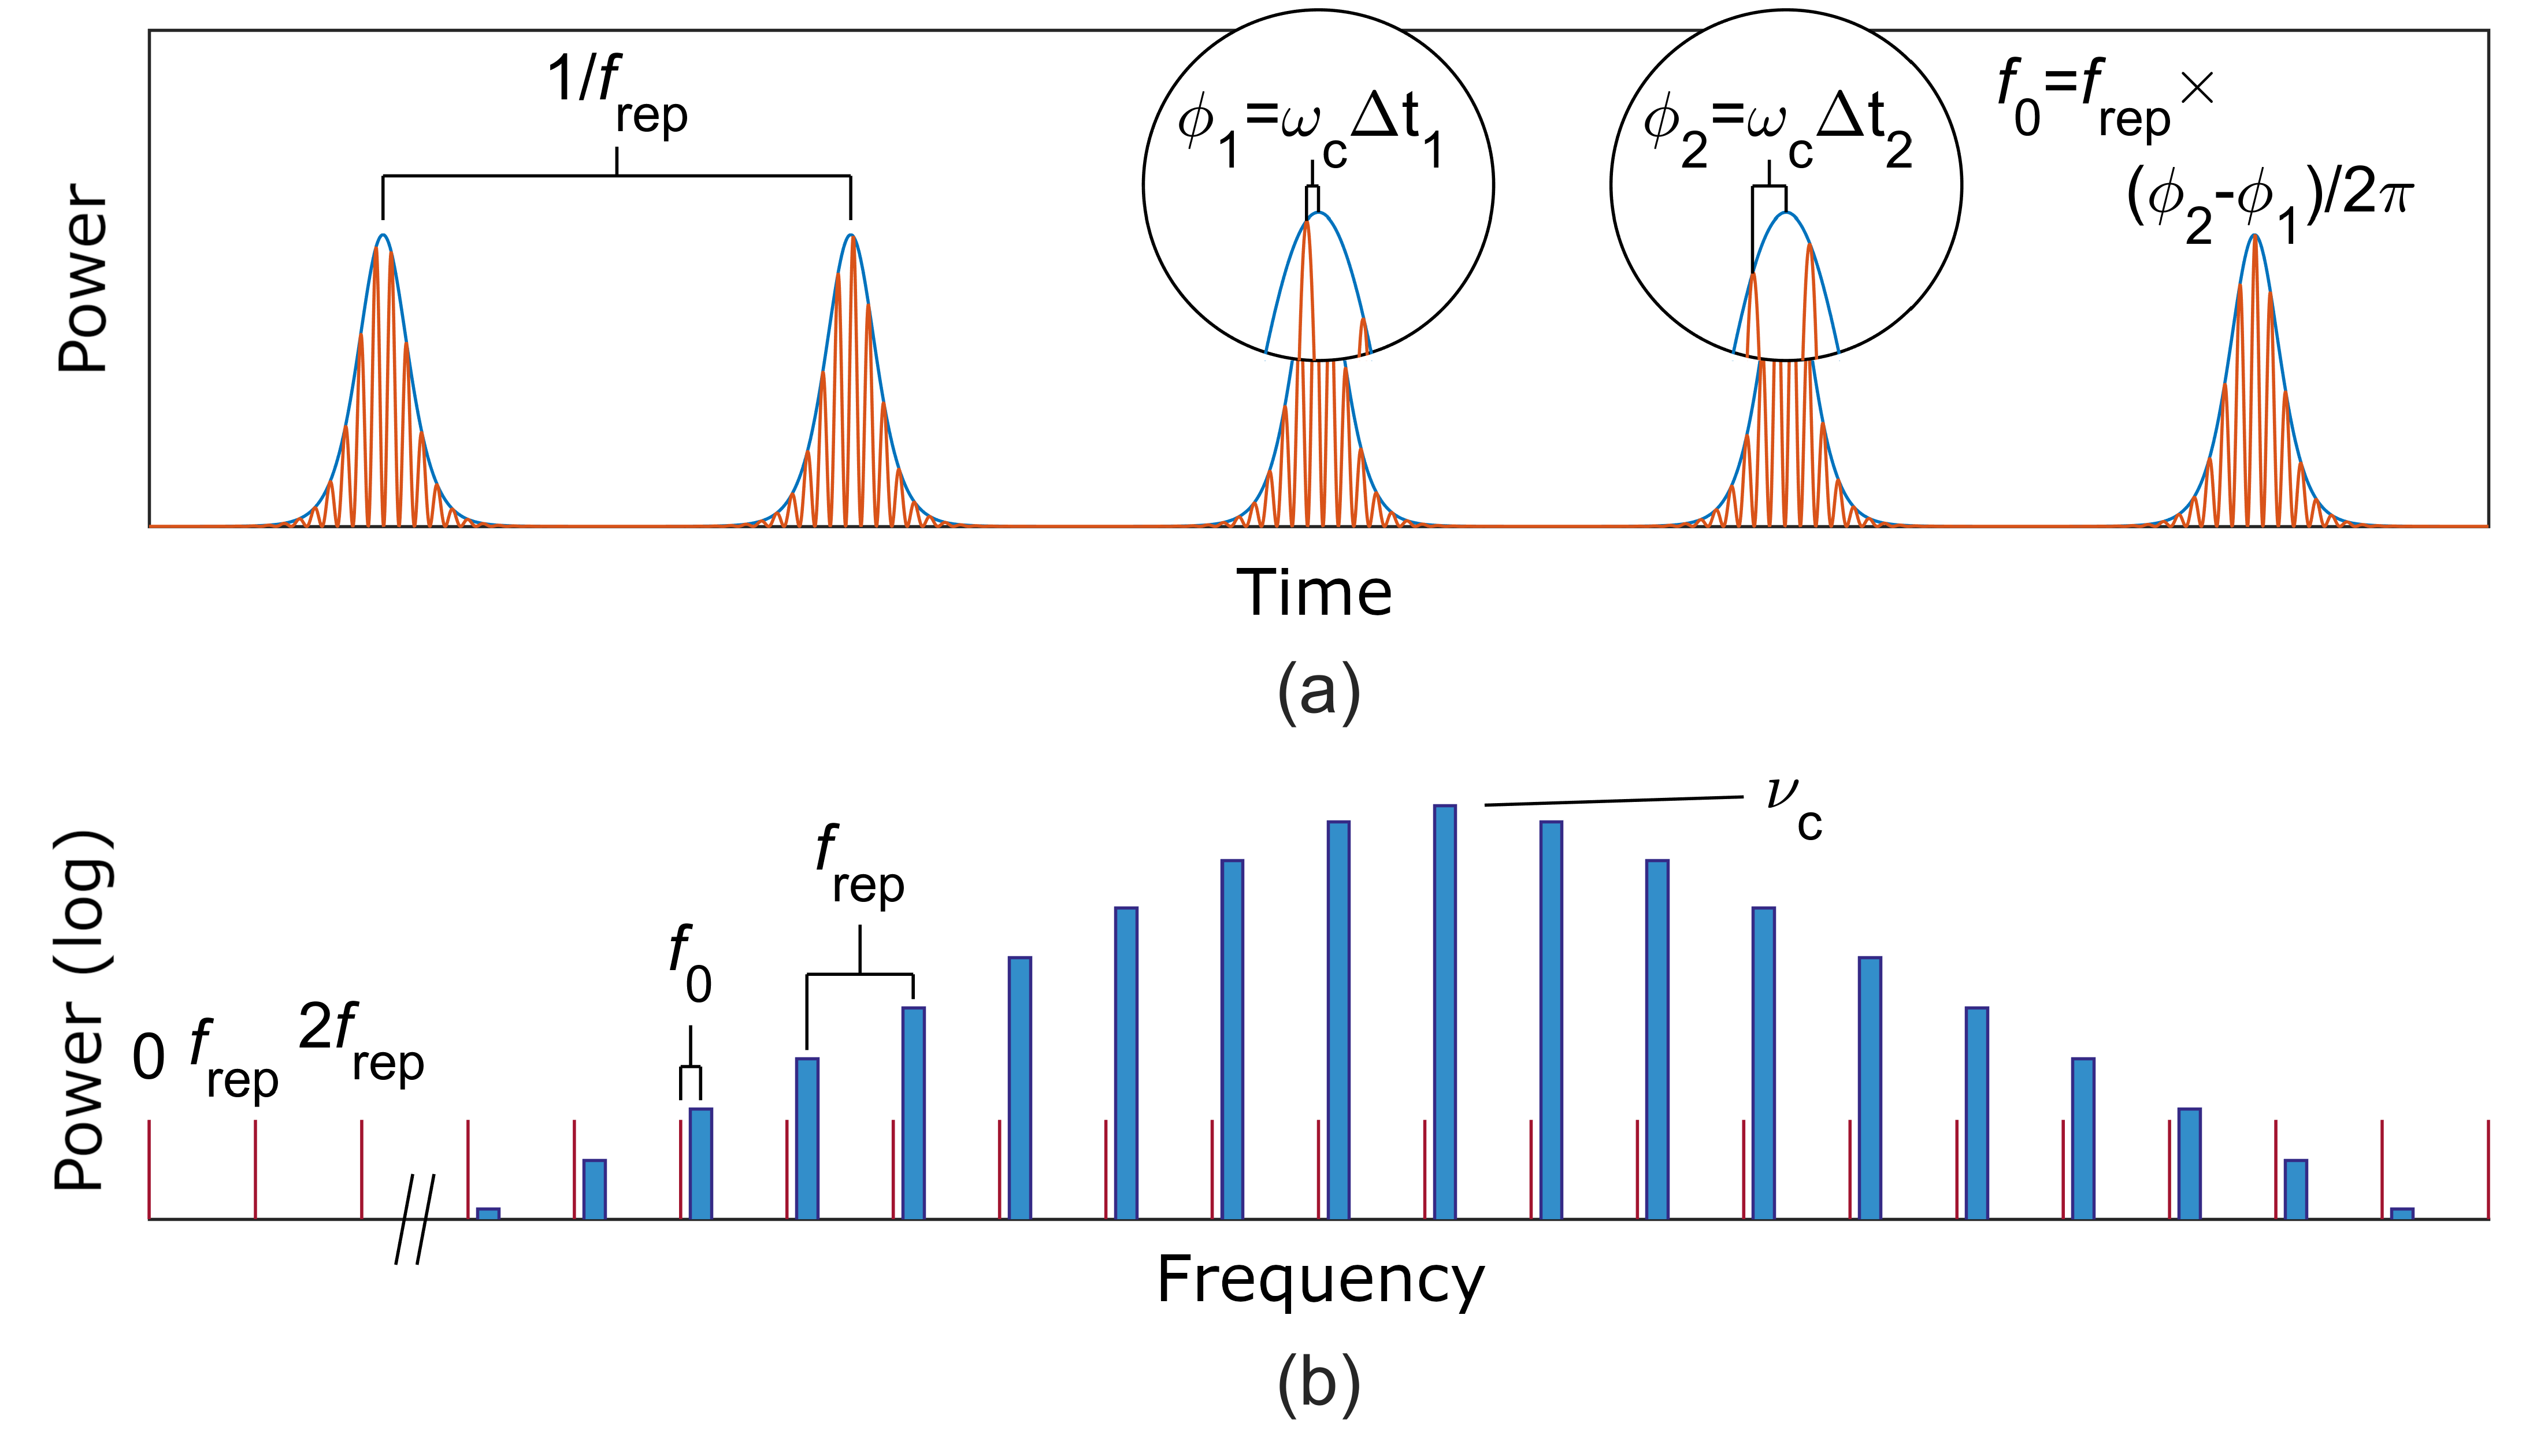
\includegraphics{\FigPath/Figures/Introduction/IntroFCbasicsv2.png}
	\end{center}
	\caption[Optical frequency combs in the time and frequency domains]{\textbf{Optical frequency combs in the time and frequency domains.} (a) Time-domain depiction of a frequency comb as a train of pulses spaced by $1/f_{rep}$. The intensity envelope is shown in blue, and the carrier wave is shown in orange. The carrier-envelope offset frequency $f_0$ arises from a phase-slip of the carrier with respect to the intensity envelope from pulse to pulse. Specifically, if phases $\phi_j=\omega_c\Delta t_j$ are traced out by the carrier wave between its maximum and the $j$\textsuperscript{th} peak of the pulse train, then $f_0=\frac{\phi_{j+1}-\phi_j}{2\pi}f_{rep}$. (b) Frequency-domain depiction of the same frequency comb. The comb modes (shown in blue) are centered around an optical frequency $\nu_c$ and offset from harmonics of the repetition rate $f_{rep}$ (shown in red) by a frequency shift $f_0$. Note that the x-axis has been broken, and the zero-referenced mode numbers of the comb modes shown are large, e.g. $n\sim19340$ for a 10 GHz repetition-rate comb centered at 1550 nm wavelength (see Chapter \ref{chap:EOMCombs}). }
	\label{fig:CombBasics}
\end{figure} 



It is useful to consider a mathematical treatment of an optical pulse train to understand the relationships presented above. In the time domain, the electric field $E(t)$ of the pulse train consists of optical pulses that arrive periodically and have baseband (centered at zero frequency) field envelope $A(t)$ multiplying the carrier wave of angular frequency $\omega_c=2\pi\nu_c$:
\begin{equation}
E(t)=\sum_{k=-\infty}^{\infty} A(t-kT)e^{i\omega_c t}. \label{eq:pulsetrain}
\end{equation}
Here, $T$ is the repetition period of the pulse train. Eq. \ref{eq:pulsetrain} can be viewed as describing a laser of angular frequency $\omega_c$ with a time-varying amplitude. This temporal modulation leads to the distribution of the power across a spectrum whose width scales inversely with the temporal duration of $A$. Intuitively, the spectrum of the comb is the spectrum of the periodic baseband field envelope\footnote{which, as the spectrum of a periodic function, is already a comb.} $\Sigma_k A(t-kT)$, shifted in frequency by the multiplication with $e^{i\omega_c t}$ so that it is centered around the optical carrier. More formally, we can calculate the frequency content of the comb by calculating
\begin{equation}
\mathcal{F}\left\{E\right\}(\omega)\sim\left(\sum_{k=-\infty}^{\infty}\mathcal{F}\left\{A(t-kT)\right\}\right)*\delta(\omega-\omega_c).
\end{equation}
Here $\mathcal{F}$ denotes Fourier transformation and $*$ denotes convolution; this expression results from the Fourier transform's property that the transform of a product is the convolution of the transforms: $\mathcal{F}(A\cdot B)=\mathcal{F}(A)*\mathcal{F}(B)$. Now we use the Fourier transform's property that a temporal translation results in a linear spectral phase shift to obtain:
\begin{equation}
\mathcal{F}\left\{E\right\}\sim\left(\mathcal{F}\left\{A\right\}\times\sum_{k=-\infty}^{\infty}e^{-i\omega kT}\right)*\delta(\omega-\omega_c).
\end{equation}
The quantity $\Sigma_ke^{-i\omega kT}$ is the Fourier-series representation of the series of $\delta$-functions \mbox{$\Sigma_\mu\delta(\omega-2\pi\mu/T)$} (the \textit{Dirac comb}), so we have
\begin{equation}
\mathcal{F}\left\{E\right\}(\omega)\sim\left(\mathcal{F}\left\{A\right\}\times\sum_{\mu=-\infty}^{\infty}\delta\left(\omega-2\pi \mu/T\right)\right)*\delta(\omega-\omega_c),
\end{equation}
and performing the convolution leads to the replacement of $\omega$ with $\omega-\omega_c$, leading to:
\begin{equation}
\mathcal{F}\left\{E\right\}\sim\sum_{\mu=-\infty}^{\infty}\delta\left(\omega-\omega_c-\mu\omega_r\right)\mathcal{F}\left\{A\right\}(\omega-\omega_c), \label{eq:combspectrum}
\end{equation}
where $\omega_{rep}=2\pi f_{rep}=2\pi/T$. This expression indicates that the spectrum of the comb has frequency content at modes $\nu_\mu=\nu_c+\mu f_{rep}$, and that their amplitudes are determined by the spectrum of the baseband field envelope, shifted up to the optical carrier frequency $\nu_c$. This is the natural formulation in the case of a comb derived from a CW laser, but it obscures the carrier-envelope offset frequency in the difference between $\nu_c$ and the nearest multiple of the repetition rate, as discussed above. In practice, if $f_{rep}$ is known, then a measurement of $f_0$ is equivalent to a measurement of the frequency of the input CW laser.


\subsection{Frequency stabilization of optical pulse trains}
\label{sec:f2f}

The scientific need for a method to measure optical frequencies motivated the development of optical frequency combs. While the measurement bandwidth of electronic frequency counters has improved since 1999, it remains limited to frequencies roughly \textit{ten thousand} times lower than the frequency of, e.g., visible red light. Frequency combs present a method for measurement of the unknown frequency $f_{opt}$ of an optical signal through heterodyne with a frequency comb---if $f_{opt}$ falls within the bandwidth of the frequency comb, then the frequency of the heterodyne between the comb and the signal is guaranteed to be less than $f_{rep}/2$. If the frequencies of the comb are known, measurement of the heterodyne with the signal reveals its frequency  $f_{opt}$, provided that the comb mode number and sign of the beat can be determined. This can be done via a wavelength measurement if sufficient precision is available, or by measuring the change $\partial f_b/\partial f_{rep}$, where $f_b$ is the measured frequency of the beat.

The utility of the optical frequency comb lies in the fact that measurement of the two frequencies $f_{rep}$ and $f_0$ is sufficient to determine the optical frequencies of all of the modes of the comb, thereby enabling frequency measurement of optical signals. Measurement of the repetition rates of optical pulse trains was possible before the realization of optical frequency comb technology, as this can be done by simply impinging the pulse train on a photodetector. Some pulse trains generated in new platforms have repetition rates too high for direct measurement in this way, but this challenge can be addressed by e.g. spectrally interleaving a lower repetition-rate comb \cite{Spencer2018,Briles2017}. In general, measurement of $f_0$ presents the more difficult challenge. It was the confluence of several technological developments around the turn of the twenty-first century that allowed detection and measurement of this frequency, thereby enabling creation of fully-stabilized modelocked-laser pulse trains: optical frequency combs.

The carrier-envelope offset frequency of a pulse train is challenging to measure because it describes evolution of the optical carrier wave underneath the intensity envelope, and therefore cannot be measured through straightforward detection of the intensity of the pulse train. Presently, the most straightforward way to measure $f_0$ is $f-2f$ \textit{self-referencing}. This can be performed only with a pulse train whose spectrum spans an octave---a factor of two in frequency. Given such an octave-spanning supercontinuum spectrum, a group of modes near mode number $N$ is frequency-doubled in a medium with the $\chi^{(2)}$ nonlinearity \cite{Boyd2003}. This frequency-doubled light is heterodyned with the native light in the supercontinuum with mode number near $2N$. The frequency of the resulting beat $f_b$ is:
\begin{align}
f_b&=f_{doubled}-f_{native}\\
&=2(Nf_{rep}+f_0)-(2Nf_{rep}+f_0)\\
&=f_0.
\end{align}
Such a scheme is implemented in an $f-2f$ \textit{interferometer}, which is depicted in Fig. \ref{fig:f2f}. Generating the necessary octave-spanning supercontinuum spectrum typically requires nonlinear spectral broadening of the pulse train after its initial generation except for in specific, carefully engineered cases (e.g. \cite{Briles2017,Fortier2003}). Achieving the required degree of spectral broadening while preserving the coherence properties of the pulse train is a significant challenge---in the past this has typically required launching a train of high energy ($\sim$1 nJ), temporally short ($\leq$ 100 fs) pulses into the spectral-broadening stage. Recent developments in nonlinear fiber and waveguide technology have relaxed these requirements slightly (e.g. Ref. \cite{Carlson2017}, also Chapter \ref{chap:EOMCombs}), but maintaining the coherence of the pulse train during spectral broadening remains an important consideration in designing optical frequency comb systems. 

The application of $f-2f$ self-referencing for full frequency-comb stabilization is discussed in Chapters \ref{chap:EOMCombs} and \ref{chap:PulsePicking}. Self-referencing of microresonator-based frequency combs is not a result presented explicitly in this thesis, but it is nonetheless a key step in the preparation of microcombs for applications and is a  motivation for the investigations into microcomb nonlinear dynamics that are presented in Chapters \ref{chap:PMPumping}-\ref{chap:FPLLE}.


\begin{figure}[htpb]
	\begin{center}
		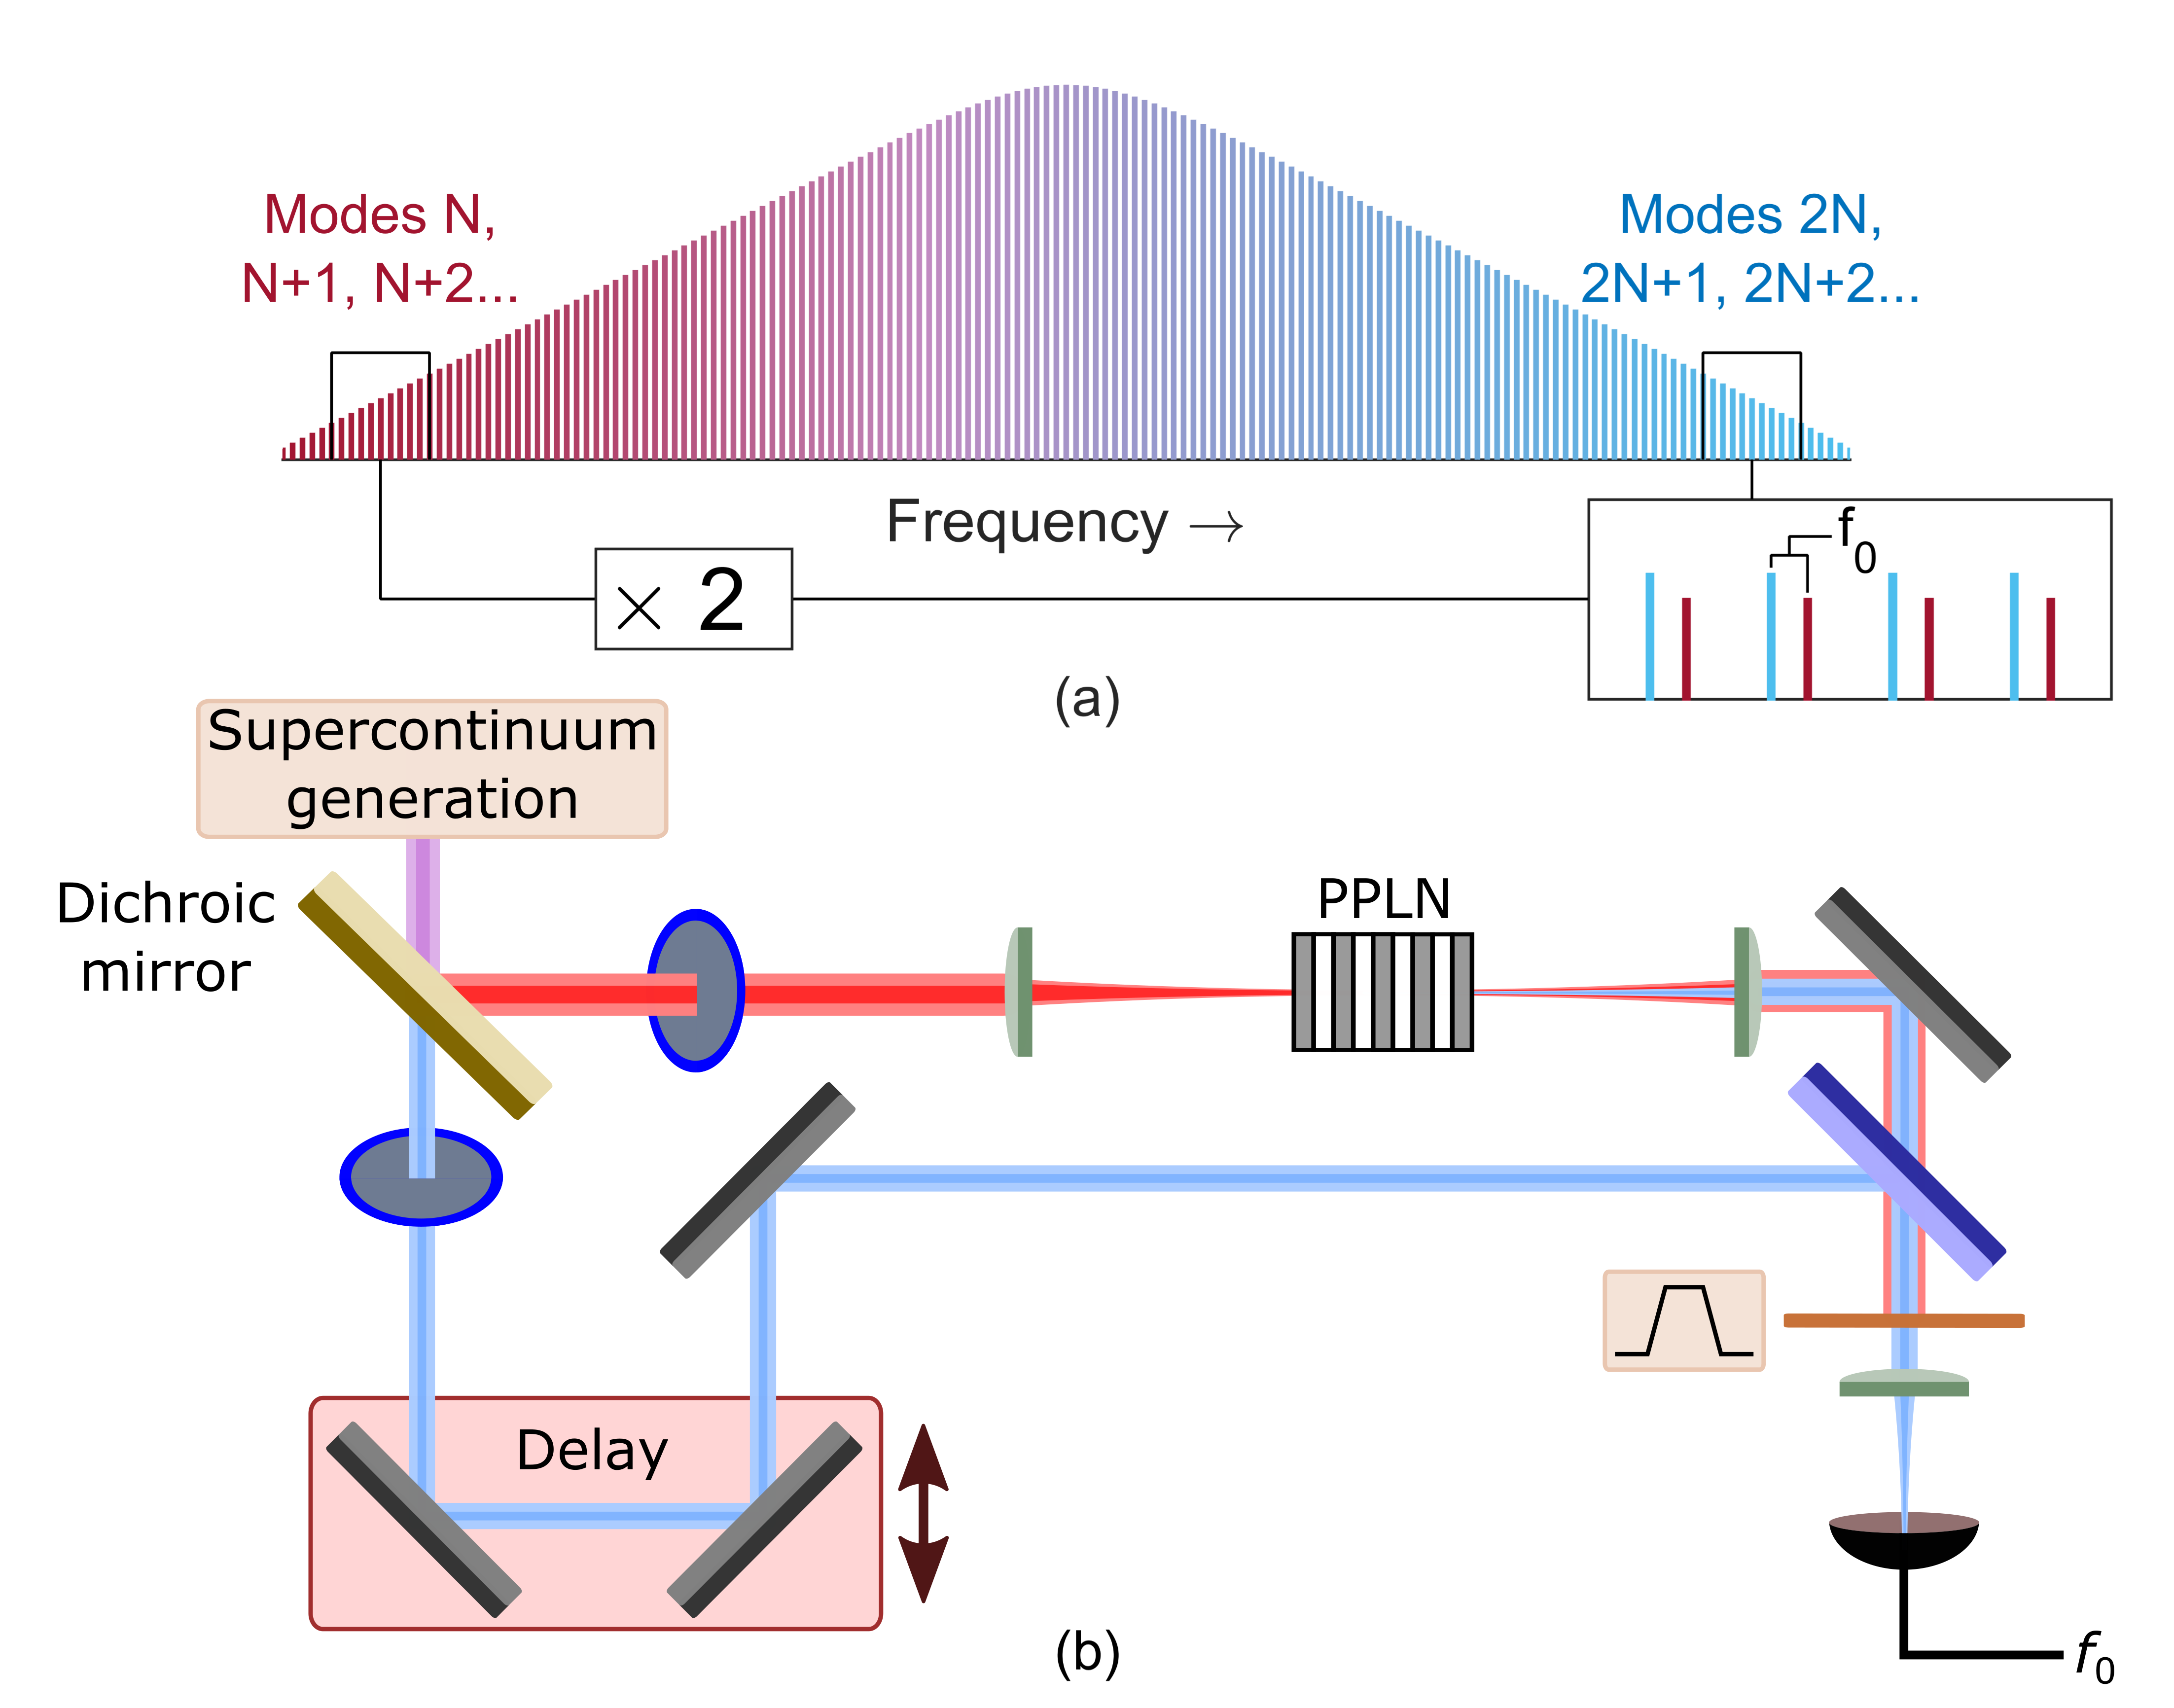
\includegraphics{\FigPath/Figures/Introduction/Introf2fv4.png}
	\end{center}
	\caption[Measurement of the carrier-envelope offset frequency via $f-2f$ self-referencing]{\textbf{Measurement of the carrier-envelope offset frequency $f_0$ via $f-2f$ self-referencing.} (a) Frequency-domain depiction of $f-2f$ self-referencing: Light on the low frequency end of an octave-spanning supercontinuum is frequency-doubled, and then heterodyned with light on the high frequency end near twice its frequency, enabling measurement of the carrier-envelope offset frequency. (b) Schematic depiction of an $f-2f$ interferometer: After supercontinuum generation, a dichroic mirror splits the light by wavelength, and the low-frequency end of the supercontinuum (red) is sent through a nonlinear crystal for frequency-doubling. Here the crystal is periodically-poled lithium niobate (PPLN), where quasi-phasematching is employed for efficient doubling of the target modes \cite{Hum2007}. The high-frequency end (blue) is sent through a delay stage, which can be adjusted to compensate for temporal walk-off between the spectral components (modes $\sim N$ and modes $\sim 2N$) required for self-referencing during the supercontinuum generation process. The two beams are then recombined by a beamsplitter and sent through a narrow optical band-pass filter centered around the doubled modes, which filters out light not necessary for $f_0$ measurement to increase the signal-to-noise ratio of the detection. Photodetection of the band-passed beam then reveals $f_0$. Waveplates in each path are used to optimize the polarization of the long-wavelength light for frequency-doubling and to ensure co-polarization of the two beams on the detector. }
	\label{fig:f2f}
\end{figure} 
